\documentclass{scrartcl}
\usepackage[utf8]{inputenc}
\usepackage{graphicx}
\usepackage{adjustbox}
\usepackage{amsmath}
\usepackage{float}
\usepackage{siunitx}
\sisetup{
  per-mode=symbol,
  separate-uncertainty
}
\usepackage{hyperref}
\hypersetup{
  colorlinks=true,
  linkcolor=blue,
  filecolor=magenta,
  urlcolor=cyan,
  pdfpagemode=FullScreen,
}
\usepackage{authblk}

\usepackage[outputdir=output]{minted}

\title{CGL-sheet11}

\author[1]{Robin Kühnberger}
\author[2]{Felix Naraschewski}

\affil[1]{University Stuttgart}
\affil[2]{University Stuttgart}

\date{\today}

\begin{document}
\maketitle
\tableofcontents

\section{Erstellen einer Vektorgrafik}

\section{Lineare Algebra mit NumPy: Fibonacci-Folge}

\inputminted[breaklines]{python3}{fibonacci.py}

\begin{figure}[H]
  \centering
  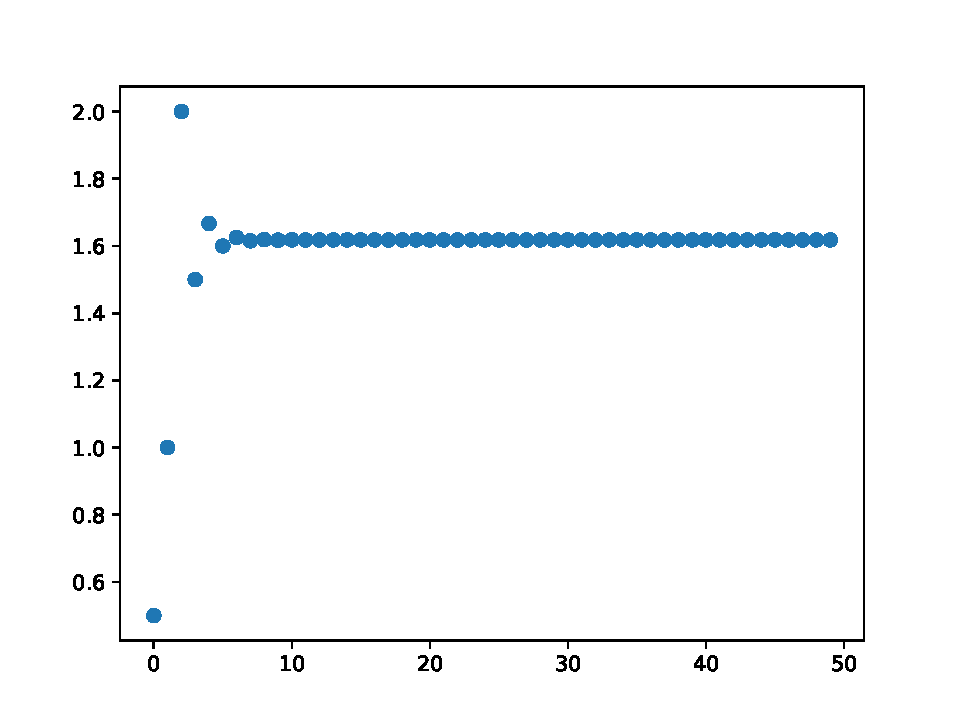
\includegraphics[width=1\textwidth]{fibonacci.pdf}
  \caption{Golden ratio}
  \label{img:01}
\end{figure}

Die Folge $\frac{a_n}{a_{n-1}}$ konvergiert für $n \to \infty$ zu $\approx 1,6180$ was dem goldenen Schnitt $\phi$ entspricht.

\section{Quicksort}
Dieses Quicksort (\href{https://de.wikipedia.org/wiki/Quicksort#Pseudocode}{Wikipedia}) benutzt ein Hoare-ähnliches Partitionieren mit zwei Zeigern, die von links und rechts aufeinander zulaufen, und versucht Elemente durch gegenseitiges Vertauschen “von beiden Seiten” um den Pivot herum anzuordnen. Bei großen $n$ treten daher Fehler auf.

\inputminted[breaklines]{python3}{quicksort.py}

Die Lomuto-Variante läuft stattdessen mit einem Zeiger durch das Intervall und hält einen zweiten Zeiger für die Grenze “alle Elemente ≤ Pivot”, wobei der Pivot am Ende immer explizit an seine endgültige Position getauscht wird und somit nach der Partition garantiert nicht mehr in einem rekursiven Aufruf vorkommt. Funktioniert auch für große $n$.

\inputminted[breaklines]{python3}{quicksort_lomuto.py}



%\section*{Quellen}
%\bibliographystyle{plain}
%\bibliography{bibliography}

\listoffigures
%\listoftables

\end{document}